In this section we investigate whether there are intrinsic time structures which might bias the signal extraction. We do this by considering 1000 iterations of the various analyses presented in section~\ref{sec:double_ratio} and \ref{sec:double_ratio_injection_studies}.

In particular, we will:
\begin{enumerate}
    \item Study the distribution of the extracted coefficients in multiple SM samples to check whether they are centered around zero.
    \item Consider one sample which yields a 3 sigma deviation from zero for one coefficient (which is to be expected when looking at 1000 samples) and scramble its time stamps 1000 times. The purpose is to see whether some memory of the 3 sigma tension remains after scrambling.
    \item We generate one sample with a sidereal signal injection and scramble its time stamps 1000 times. This is a test for partial unblinding of the data.
    \item We generate 1000 injected samples (with the same coefficient) and study each one of them over a range of testing phases. We then look at the average of the extracted coefficient for each testing phase. This will produce a ``chirp'' structure (in the testing phase vs fitted coefficient plane). When looking at a given sample, the fitted coefficients will lie on a ``sampled'' version of this curve. 
\end{enumerate}

\subsection{SM simulation: multiple samples}
\label{ssec:SM_1000}
%
We repeated 1000 times the analysis presented in section~\ref{ssec:all_errors_included} with the purpose of checking whether the fitted coefficients are distributed around zero. This is indeed the case as can be seen in figure~\ref{fig:SM_1000}. In the figures we display both the average uncertainty of the fitted values ($\langle \delta d_u^{YZ} \rangle$) and the standard deviation of the central values ($\sigma ([d_u^{YZ}]_\text{CV})$). The (expected) agreement between the two signal a nice Gaussian distribution of the results. This agreement persists for all other coefficiences (not shown).

In figures~\ref{fig:SM_1000_fits_sidsol} and \ref{fig:SM_1000_fits_1h} we show the average and standard deviations for all fitted coefficients. We see that they are all strictly centered at zero.

\begin{figure}[H]
\centering
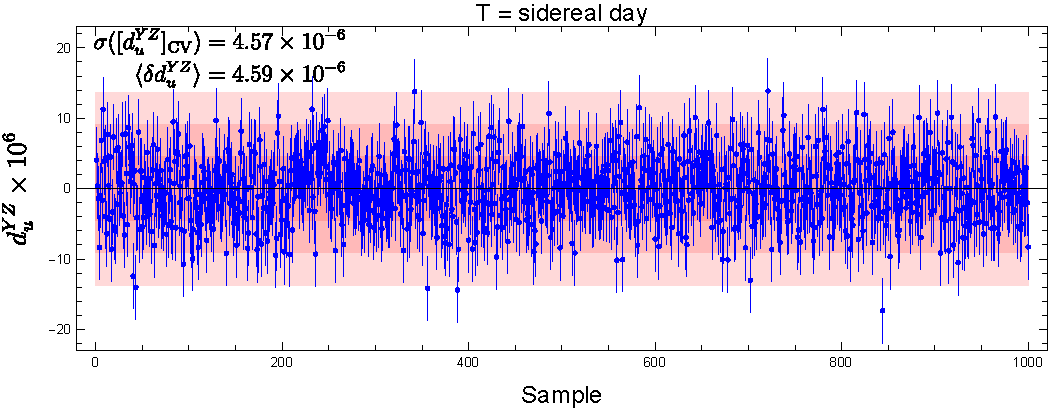
\includegraphics[width=\textwidth]{figs/Mathematica-oldchi2/fit_duYZ_SM_1000samples_sday}
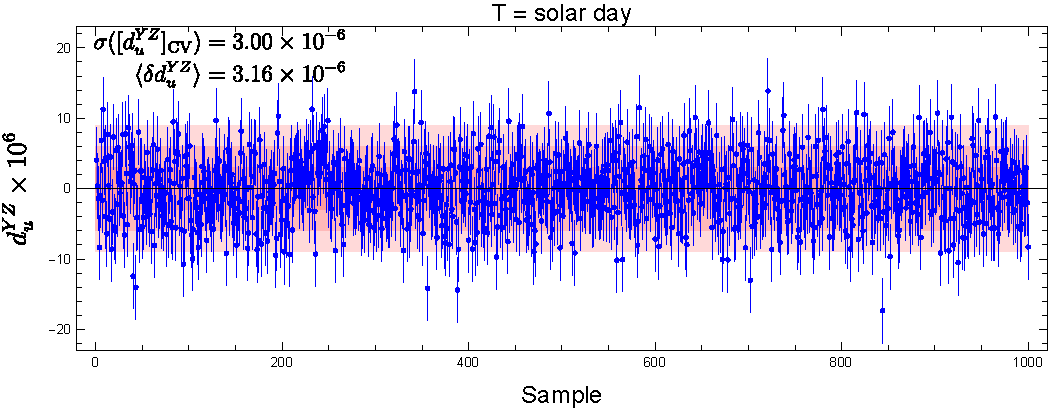
\includegraphics[width=\textwidth]{figs/Mathematica-oldchi2/fit_duYZ_SM_1000samples_day}
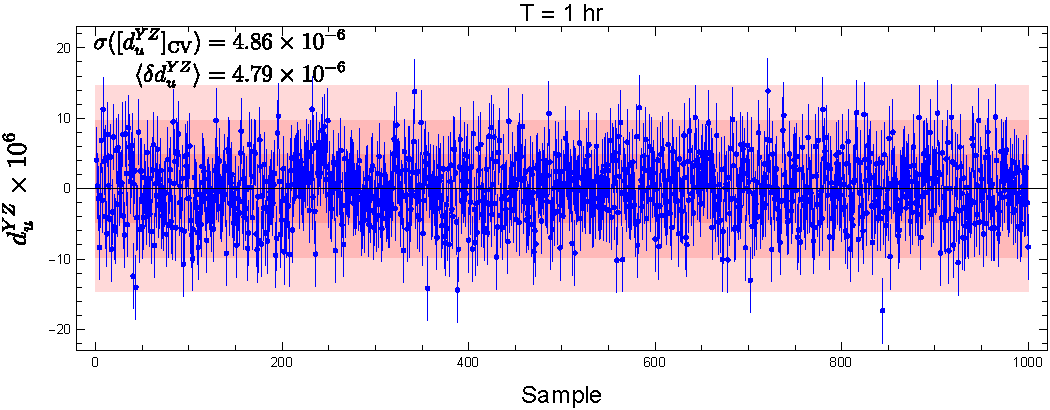
\includegraphics[width=\textwidth]{figs/Mathematica-oldchi2/fit_duYZ_SM_1000samples_1}
\caption{Distribution of the fitted coefficient $d_u^{YZ}$ extracted from 1000 SM samples. The three panels correspond to sidereal, solar and 1 hr testing phases. \textcolor{red}{The solar distribution seems too narrow. }}
\label{fig:SM_1000}
\end{figure} 


\begin{figure}[H]
\centering
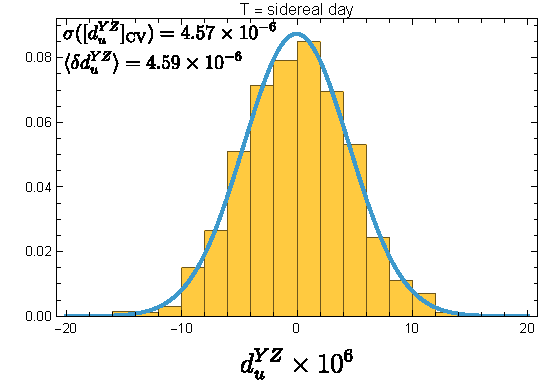
\includegraphics[width=.32\textwidth]{figs/Mathematica-oldchi2/fit_duYZ_SM_1000samples_sday_hist}
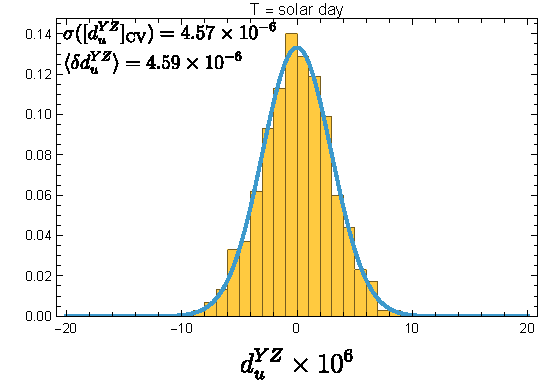
\includegraphics[width=.32\textwidth]{figs/Mathematica-oldchi2/fit_duYZ_SM_1000samples_day_hist}
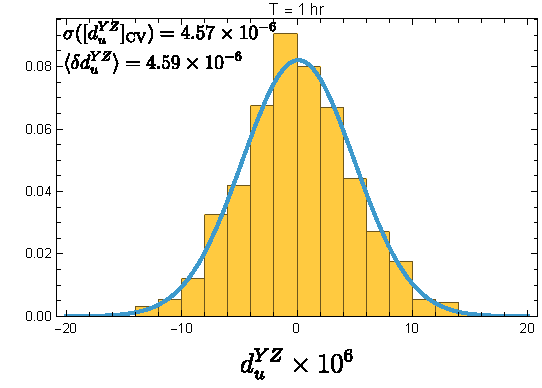
\includegraphics[width=.32\textwidth]{figs/Mathematica-oldchi2/fit_duYZ_SM_1000samples_1_hist}
\caption{Histogram of the distribution of the fitted coefficient $d_u^{YZ}$ extracted from 1000 SM samples. The three panels correspond to sidereal, solar and 1 hr testing phases. \textcolor{red}{The solar distribution seems too narrow. }}
\label{fig:SM_1000_hist}
\end{figure} 




\begin{figure}[H]
\centering
\begin{minipage}[H]{\textwidth}
    \vspace{0pt}
    \centering
   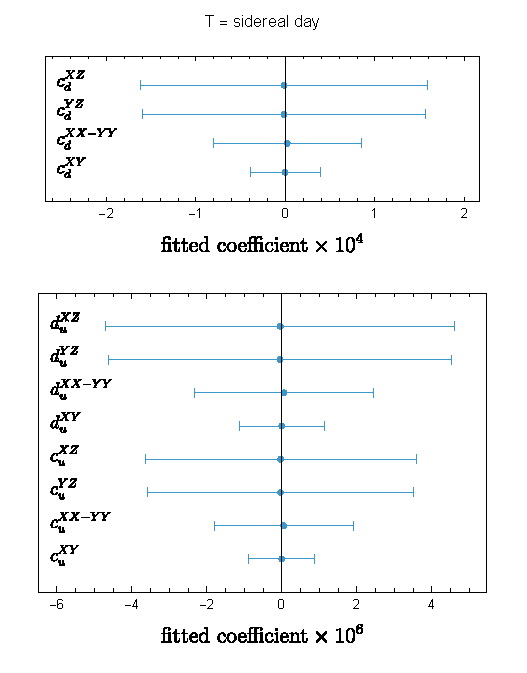
\includegraphics[width=0.49\textwidth]{figs/Mathematica-oldchi2/fit_duYZ_SM_1000samples_sday_fit}
   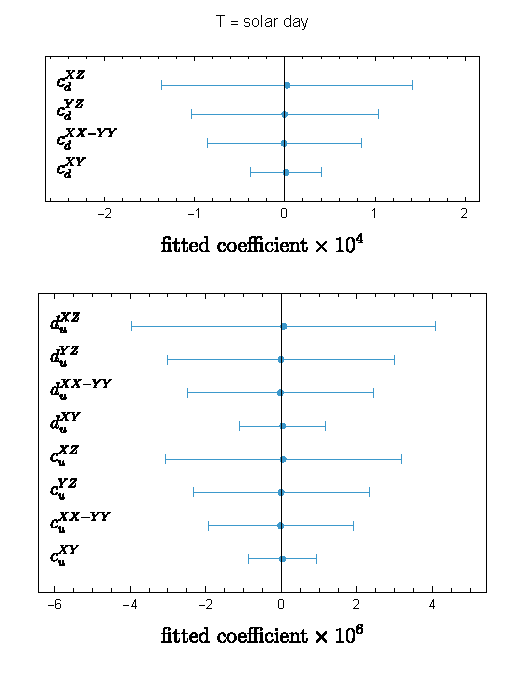
\includegraphics[width=0.49\textwidth]{figs/Mathematica-oldchi2/fit_duYZ_SM_1000samples_day_fit}
\end{minipage}
\begin{minipage}[H]{\textwidth}
    \vspace{1.6cm}
    \centering
    \begin{tabular}{|l|c|}
        \hline
$d_u^{XZ}$ & $(0. \pm 4.6)\times 10^{-6}$ \\
$d_u^{YZ}$ & $(-0. \pm 4.6)\times 10^{-6}$ \\
$d_u^{XX-YY}$ & $(0. \pm 2.4)\times 10^{-6}$ \\
$d_u^{XY}$ & $(0. \pm 11.)\times 10^{-7}$ \\
$c_u^{XZ}$ & $(0. \pm 3.6)\times 10^{-6}$ \\
$c_u^{YZ}$ & $(-0. \pm 3.5)\times 10^{-6}$ \\
$c_u^{XX-YY}$ & $(0. \pm 1.9)\times 10^{-6}$ \\
$c_u^{XY}$ & $(0. \pm 8.8)\times 10^{-7}$ \\
$c_d^{XZ}$ & $(0. \pm 1.6)\times 10^{-4}$ \\
$c_d^{YZ}$ & $(-0. \pm 1.6)\times 10^{-4}$ \\
$c_d^{XX-YY}$ & $(0.2 \pm 8.3)\times 10^{-5}$ \\
$c_d^{XY}$ & $(0. \pm 3.9)\times 10^{-5}$ \\
                \hline
        \end{tabular}
        \;\;\;\;\;\;\;\;\;\;\;\;\;\;\;\;\;\;
    \begin{tabular}{|l|c|}
        \hline
$d_u^{XZ}$ & $(0. \pm 4.0)\times 10^{-6}$ \\
$d_u^{YZ}$ & $(0. \pm 3.0)\times 10^{-6}$ \\
$d_u^{XX-YY}$ & $(-0. \pm 2.5)\times 10^{-6}$ \\
$d_u^{XY}$ & $(0. \pm 11.)\times 10^{-7}$ \\
$c_u^{XZ}$ & $(0. \pm 3.1)\times 10^{-6}$ \\
$c_u^{YZ}$ & $(0. \pm 2.3)\times 10^{-6}$ \\
$c_u^{XX-YY}$ & $(-0. \pm 1.9)\times 10^{-6}$ \\
$c_u^{XY}$ & $(0.3 \pm 8.9)\times 10^{-7}$ \\
$c_d^{XZ}$ & $(0. \pm 1.4)\times 10^{-4}$ \\
$c_d^{YZ}$ & $(0. \pm 1.0)\times 10^{-4}$ \\
$c_d^{XX-YY}$ & $(-0. \pm 8.5)\times 10^{-5}$ \\
$c_d^{XY}$ & $(0.1 \pm 3.9)\times 10^{-5}$ \\
                        \hline
        \end{tabular}
\end{minipage}
\caption{Sidereal signal injection test ($d_u^{YZ} = 1.35 \times 10^{-4}$): fit results for sidereal (left) and solar (right) testing phases.}
\label{fig:SM_1000_fits_sidsol}
\end{figure}


\begin{figure}[H]
\centering
\begin{minipage}[H]{0.49\textwidth}
    \vspace{1.6cm}
    \centering
    \begin{tabular}{|l|c|}
        \hline
$d_u^{XZ}$ & $(0.3 \pm 4.9)\times 10^{-6}$ \\
$d_u^{YZ}$ & $(0.1 \pm 4.9)\times 10^{-6}$ \\
$d_u^{XX-YY}$ & $(-0. \pm 2.4)\times 10^{-6}$ \\
$d_u^{XY}$ & $(0. \pm 12.)\times 10^{-7}$ \\
$c_u^{XZ}$ & $(0.2 \pm 3.8)\times 10^{-6}$ \\
$c_u^{YZ}$ & $(0. \pm 3.8)\times 10^{-6}$ \\
$c_u^{XX-YY}$ & $(-0. \pm 1.9)\times 10^{-6}$ \\
$c_u^{XY}$ & $(0.3 \pm 9.6)\times 10^{-7}$ \\
$c_d^{XZ}$ & $(0. \pm 1.7)\times 10^{-4}$ \\
$c_d^{YZ}$ & $(0. \pm 1.7)\times 10^{-4}$ \\
$c_d^{XX-YY}$ & $(-0.1 \pm 8.3)\times 10^{-5}$ \\
$c_d^{XY}$ & $(0.1 \pm 4.3)\times 10^{-5}$ \\
        \hline
        \end{tabular}
\end{minipage}
\begin{minipage}[H]{0.49\textwidth}
    \vspace{0pt}
    \centering
   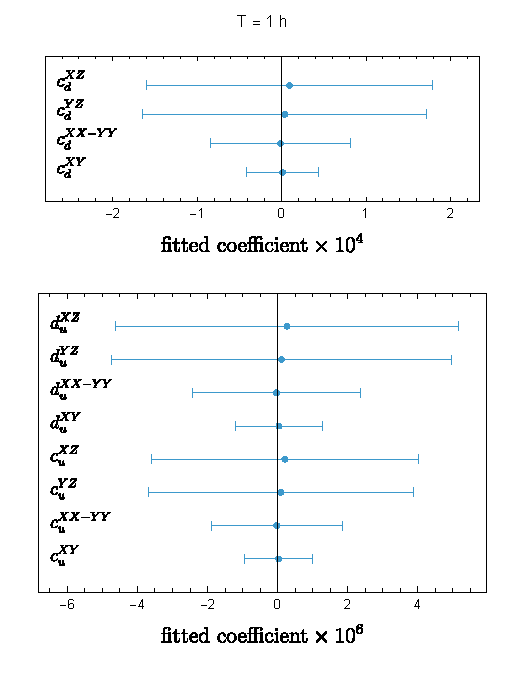
\includegraphics[width=\textwidth]{figs/Mathematica-oldchi2/fit_duYZ_SM_1000samples_1_fit}
\end{minipage}
\caption{Sidereal signal injection test ($d_u^{YZ} = 1.35 \times 10^{-4}$): fit results for 1 hr testing phase.}
\label{fig:SM_1000_fits_1h}
\end{figure}


\subsection{Multiple time scramblings of ``bad'' sample}
\label{ssec:bad_sample}
%
In this section we select one of the samples we generated in section~\ref{ssec:SM_1000} for a which the fitted value of a coefficient deviates from zero at the three sigma level. Sample \#844 yields a $3.8\;\sigma$ tension: $\left[d_u^{YZ}\right]_\text{fit} = -(1.73 \pm 0.46) \times 10^{-5}$. Note that this is not an anomaly but simply a statistical necessity given the number of the generated samples. The question is whether multiple scramblings of this sample will retain a memory of this tension. The result of this study is presented in figure~\ref{fig:SM_1000_bad_sample}, from which we see that no memory of the initial tension remains in the 1000 successive scramblings. 

\begin{figure}[H]
\centering
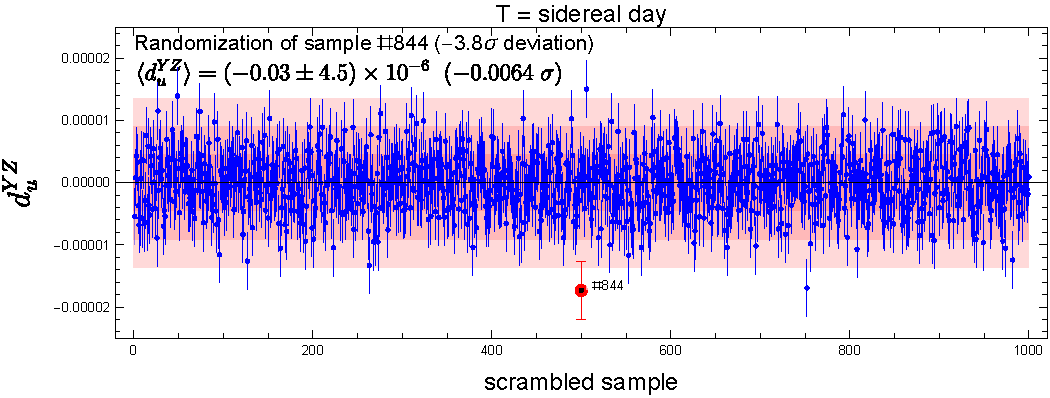
\includegraphics[width=\textwidth]{figs/Mathematica-oldchi2/fit_duYZ_SM_sample844_1000scrambles}
\caption{1000 scramblings of sample \#844 which displays an accidental 3.8 sigma tension.}
\label{fig:SM_1000_bad_sample}
\end{figure}


\subsection{Multiple time scramblings of an injected signal}
\label{ssec:signal_1000scramblings}
%
In this test, we inject a $d_u^{YZ} = 1.35 \times 10^{-4}$ signal. Typically this signal will yield results like those presented in section~\ref{ssec:SiderealInjectionRecovery} (figures~\ref{fig:RD_sidereal_signal} and \ref{fig:RD_sidereal_signal_fits_sidsol}). Here we consider 1000 scrambles of the time stamps of this sample and perform a sidereal time analysis. The purpose of this is to show that no memory of the signal remains. The result of this study is presented in figure~\ref{fig:sidereal_signal_1000_scrambles}.

\begin{figure}[H]
\centering
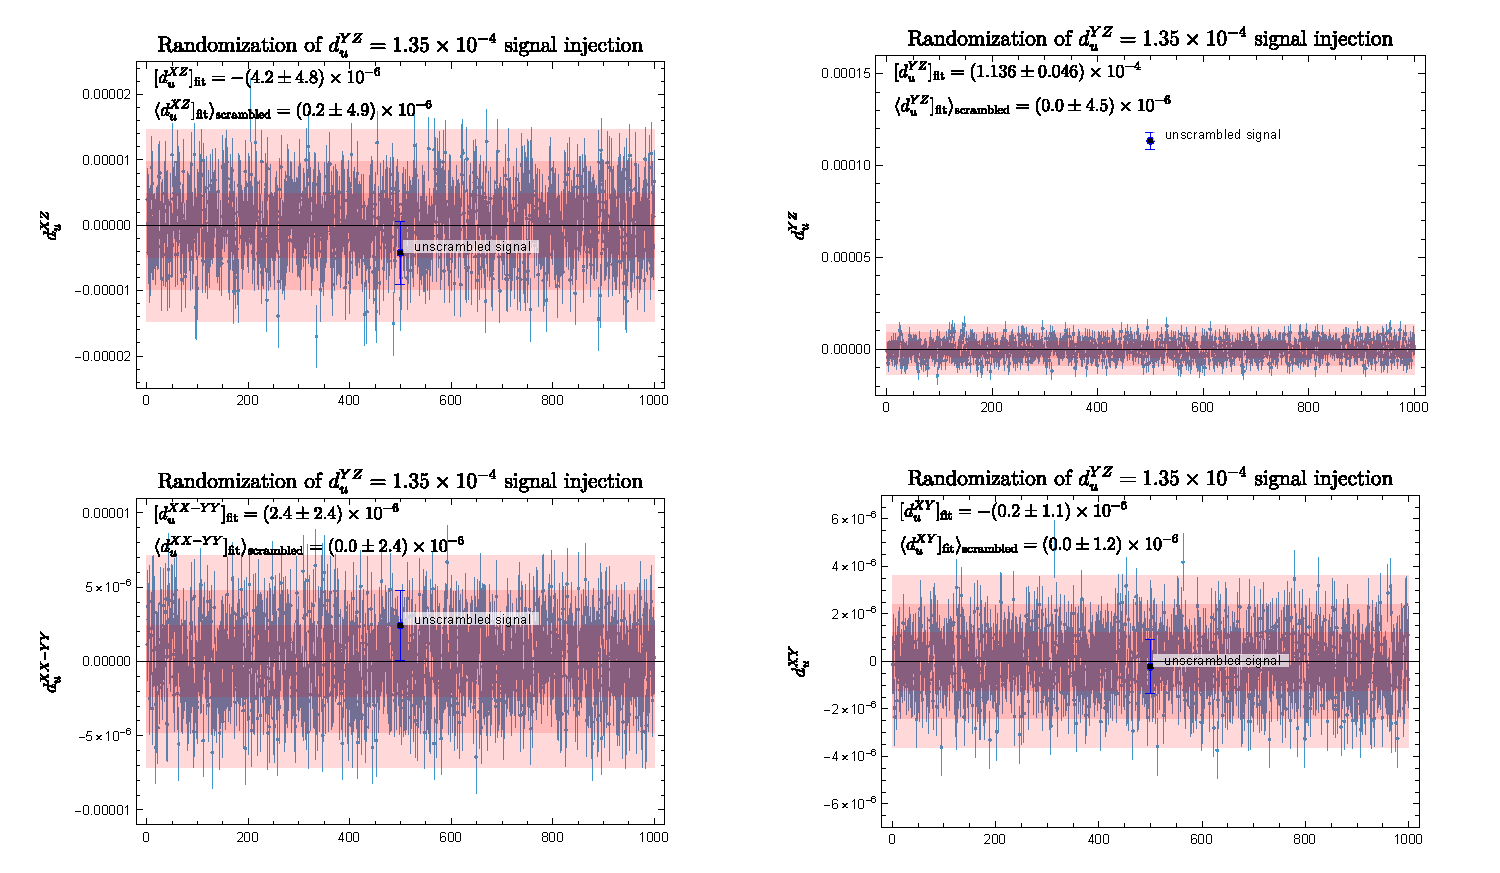
\includegraphics[width=\textwidth]{figs/Mathematica-oldchi2/fit_duYZinjected_1000scrambles}
\caption{Distribution of the fitted coefficient $d_u^{YZ}$ obtained by scrambling 1000 times the time stamps of an injected signal. }
\label{fig:sidereal_signal_1000_scrambles}
\end{figure}


\subsection{Multiple samples of an injected signal analyzed over a range of testing phases}
\label{ssec:signal_1000samples_phasesscan}
%
In this section, we inject a $d_u^{YZ} = 1.35 \times 10^{-4}$ signal and generate 1000 samples. Each sample is than analyzed over a range of testing phases. For each testing phase we then average the 1000 fit outcomes. The results of this analysis are presented in figures~\ref{fig:sidereal_signal_1000_scrambles_scan_wide} and \ref{fig:sidereal_signal_1000_scrambles_scan_narrow}. The results we obtain for the sidereal, solar and 1 hr testing phases are summarized in figure~\ref{fig:sidereal_signal_1000_scrambles_scan_fit}. The ``chirp'' structures that we observe in figure~\ref{fig:sidereal_signal_1000_scrambles_scan_narrow} are not affected by the Poisson/Gaussian sampling and are a reflection of the intrinsic time structure of the data. 

\begin{figure}[H]
\centering
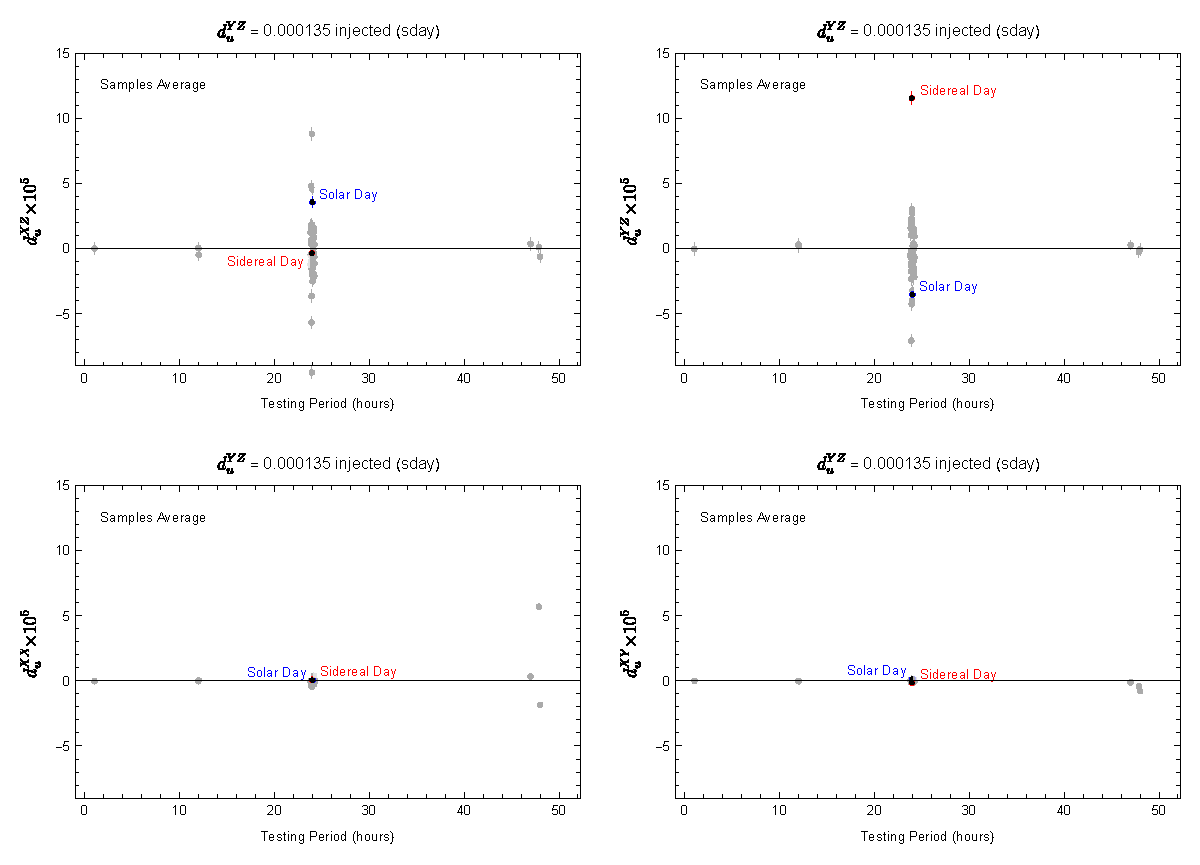
\includegraphics[width=\textwidth]{figs/Mathematica-oldchi2/fit_duYZinjected_1000samples_phasescan_wide}
\caption{Averages (over 1000 injections of a $d_u^{YZ} = 1.35 \times 10^{-4}$ sidereal signal) of the fit results for various SME coefficients as a function of the testing phase.}
\label{fig:sidereal_signal_1000_scrambles_scan_wide}
\end{figure}

\begin{figure}[H]
\centering
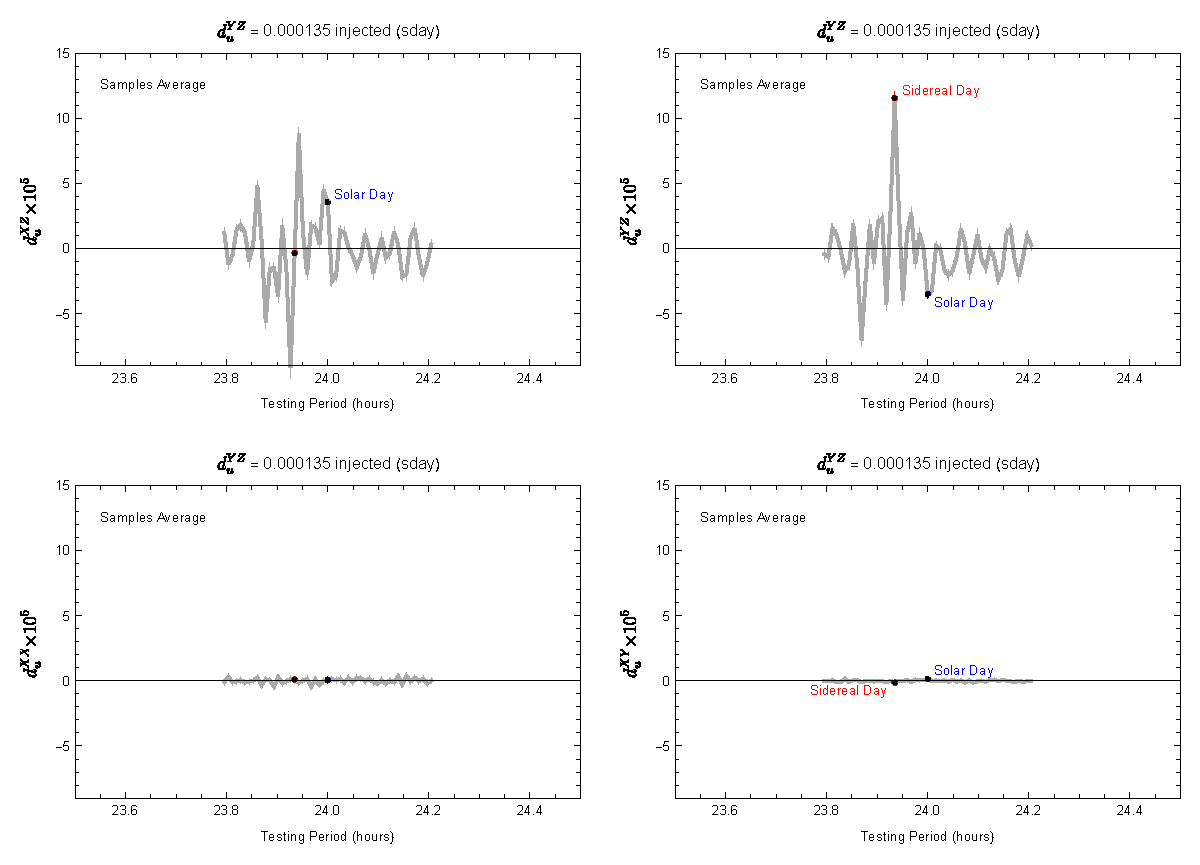
\includegraphics[width=\textwidth]{figs/Mathematica-oldchi2/fit_duYZinjected_1000samples_phasescan_narrow}
\caption{Averages (over 1000 injections of a $d_u^{YZ} = 1.35 \times 10^{-4}$ sidereal signal) of the fit results for various SME coefficients as a function of the testing phase (zoom).}
\label{fig:sidereal_signal_1000_scrambles_scan_narrow}
\end{figure}



\begin{figure}[H]
\centering
\begin{minipage}[H]{0.49\textwidth}
    \vspace{0pt}
    \centering
   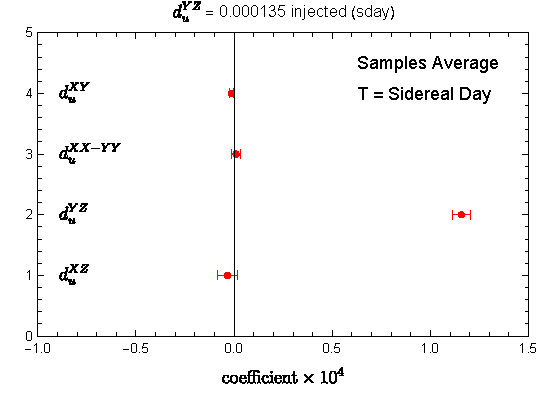
\includegraphics[width=\textwidth]{figs/Mathematica-oldchi2/fit_duYZinjected_1000samples_averages_sday}
\end{minipage}
\begin{minipage}[H]{0.49\textwidth}
    \vspace{0pt}
    \centering
 \begin{tabular}{|l|c|}
        \hline
        $d_u^{XY}$ & $ (-1.4 \pm 1.1)\times 10^{-6}$ \\
        $d_u^{XX-YY}$ & $ (1. \pm 2.3)\times 10^{-6}$ \\
        $d_u^{YZ}$ & $ (1.158 \pm 0.047)\times 10^{-4}$ \\
        $d_u^{XZ}$ & $ (-3.4 \pm 5.0)\times 10^{-6}$ \\
        \hline
    \end{tabular}
\end{minipage}
\begin{minipage}[H]{0.49\textwidth}
    \vspace{0pt}
    \centering
   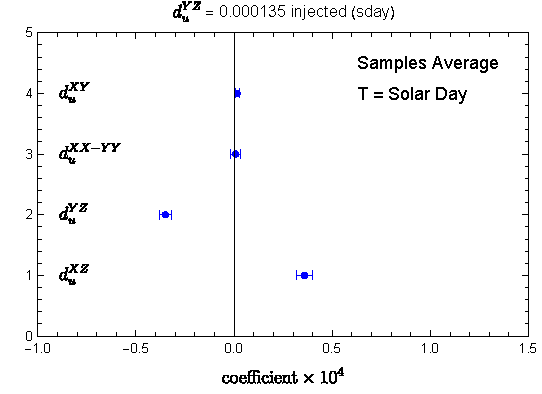
\includegraphics[width=\textwidth]{figs/Mathematica-oldchi2/fit_duYZinjected_1000samples_averages_day}
\end{minipage}
\begin{minipage}[H]{0.49\textwidth}
    \vspace{0pt}
    \centering
    \begin{tabular}{|l|c|}
        \hline
        $d_u^{XY}$ & $ (1.6 \pm 1.1)\times 10^{-6}$ \\
        $d_u^{XX-YY}$ & $ (0.7 \pm 2.4)\times 10^{-6}$ \\
        $d_u^{YZ}$ & $ (-3.50 \pm 0.32)\times 10^{-5}$ \\
        $d_u^{XZ}$ & $ (3.6 \pm 0.40)\times 10^{-5}$ \\
        \hline
        \end{tabular}
\end{minipage}
\begin{minipage}[H]{0.49\textwidth}
    \vspace{0pt}
    \centering
   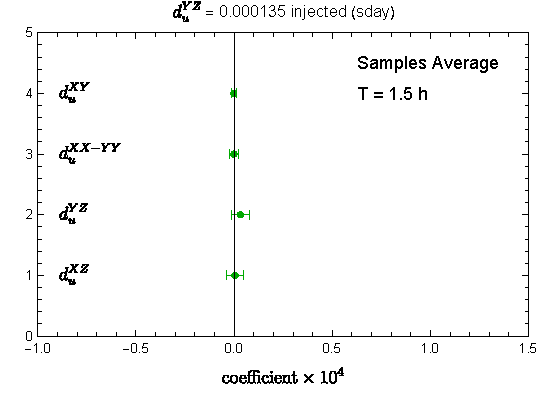
\includegraphics[width=\textwidth]{figs/Mathematica-oldchi2/fit_duYZinjected_1000samples_averages_1.5}
\end{minipage}
\begin{minipage}[H]{0.49\textwidth}
    \vspace{0pt}
    \centering
    \begin{tabular}{|l|c|}
        \hline
        $d_u^{XY}$ & $ (0.03 \pm 1.2)\times 10^{-6}$ \\
        $d_u^{XX-YY}$ & $ (-0.2 \pm 2.4)\times 10^{-6}$ \\
        $d_u^{YZ}$ & $ (-0.2 \pm 4.7)\times 10^{-6}$ \\
        $d_u^{XZ}$ & $ (0.1 \pm 4.8)\times 10^{-6}$ \\
        \hline
        \end{tabular}
\end{minipage}
\caption{Sidereal signal injection test ($d_u^{YZ} = 1.35 \times 10^{-4}$): fit results for sidereal (left) and solar (right) testing phases.}
\label{fig:sidereal_signal_1000_scrambles_scan_fit}
\end{figure}


